The transform between joint adjacent joints is represented by the transform:

\begin{equation}\label{eq:dhT}
T_i^{i-1} = \left[ \begin{array}{cccc} 
cos(\theta_i) & -sin(\theta_i)cos(\alpha_i) &  sin(\theta_i)sin(\alpha_i)  &  a_i cos(\theta_i) \\ 
sin(\theta_i) &  cos(\theta_i)cos(\alpha_i) & -cos(\theta_i)sin(\alpha_i)  &  a_i sin(\theta_i) \\
0             &  sin(\alpha_i)              &  cos(\alpha_i)               &  d_i               \\
0             &  0                          &  0                           &  1                 
\end{array} \right]
\end{equation}

Where $\theta_i$ is the 

\begin{figure}[thpb]
  \centering
%  \begin{minipage}{\textwidth}
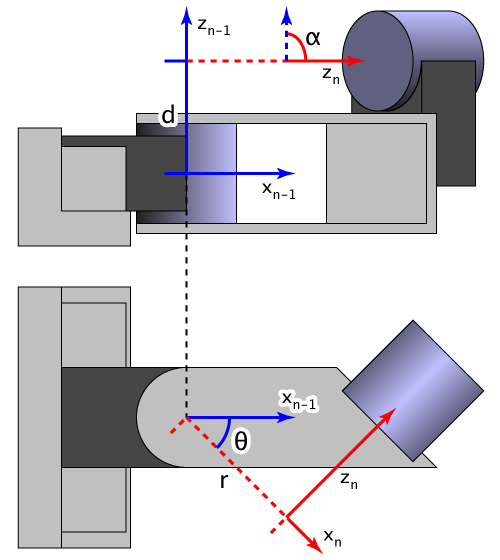
\includegraphics[width=0.5\columnwidth]{./examples/pix/Sample_Denavit-Hartenberg_Diagram.png}
\caption{Denavit-Hartenberg diagram showing that axis of rotations and displacements to create the transform in Equation~\ref{eq:dhT}.}
Image Credit: \textit{http://en.wikipedia.org/wiki/File:Sample\_Denavit-Hartenberg\_Diagram.png}
%  \end{minipage}
\end{figure}
